\documentclass[11p, titlepage, oneside, a4paper]{article}
% Packages
\usepackage{amsmath}
\usepackage{graphicx}
\usepackage{hyperref}
\usepackage[english,swedish]{babel}
\usepackage[
    backend=biber,
    style=authoryear-ibid,
    sorting=ynt
]{biblatex}
\usepackage[utf8]{inputenc}
\usepackage[T1]{fontenc}
\usepackage{booktabs}
%Källor
\addbibresource{mall.bib}
\graphicspath{ {./images/} }

% Ändra de rader som behöver ändras
\def\inst{Teknikprogrammet}
\def\typeofdoc{Laborationsrapport}
\def\course{Fysik 1 150p}
\def\pretitle{Laboration 2}
\def\title{Fjäderkraft och friktion}
\def\name{Oscar Tafvelin}
\def\username{oscar.tafvelin}
\def\email{\username{}@elev.ga.ntig.se}
\def\graders{Magnus Silverdal}

\begin{document}

\begin{titlepage}
		\thispagestyle{empty}
		\begin{large}
			\begin{tabular}{@{}p{\textwidth}@{}}
				\textbf{NTI gymnasiet \hfill \today} \\
				\textbf{\inst} \\
				\textbf{\typeofdoc} \\
			\end{tabular}
		\end{large}
		\vspace{10mm}
		\begin{center}
			\LARGE{\pretitle} \\
			\huge{\textbf{\course}}\\
			\vspace{10mm}
			\LARGE{\title} \\
			\vspace{15mm}
			\begin{large}
				\begin{tabular}{ll}
					\textbf{Namn} & \name \\
					\textbf{E-mail} & \texttt{\email} \\
				\end{tabular}
			\end{large}
			\vfill
            
\includegraphics[width=0.5\textwidth]{images/NTI Gymnasiet_Symbol_print_svart.png}
			\vfill
            \large{\textbf{Handledare}}\\
			\mbox{\large{\graders}}
		\end{center}
	\end{titlepage}

    \begin{otherlanguage}{english}
	\begin{abstract}
        We were given the task to perform two seperate experiments. During the first experiment we needed to examine which factors would effect the friction of an object. We did this by using a real model, which consisted of a plank which we used as a inclined plane. We then took a block of wood and put it on this plank and tilted one end of the plank upwards until the block of wood started sliding with a constant speed (no acceleration). After this we measured how high up the plank had to be for this to occur which we could later use in our calculations to determine the amount of friction force and normal force the block of wood was subjected to. The experiment was repeated several times with different weights on top of the block. In the other experiment we were tasked with examining the amount of force a spring was subjected to. For this we used a real model, which consisted of a retort stand which held a spring. We then hanged a series of weights on the spring and measured the length of the spring after each weight added. After both of the experiments the measurements were written down and put in their respective formulas to calculate the results.
    \end{abstract}
    \end{otherlanguage}
    % Om arbetet är långt har det en innehållsförteckning, annars kan den utelämnas
	\pagenumbering{roman}
	\tableofcontents
	
	% och lägger in en sidbrytning
	\newpage

	\pagenumbering{arabic}
	
	% i Sverige har vi normalt inget indrag vid nytt stycke
	\setlength{\parindent}{0pt}
	% men däremot lite mellanrum
	\setlength{\parskip}{10pt}
	
	\section{Syfte och frågeställning}
		Syftet med laborationen är att analysera friktionen hos ett träblock som glider nedför ett plan och att analysera fjäderkraften hos en fjäder som hängdes från ett stativ med en laboratorieklämma. Vi vill få reda på friktionskraften och normalkraften hos träblocket och fjäderkraften hos fjädern när olika mängder vikter sätts på varje experiment.

	\section{Bakgrund och teori}
        Med utgångspunkt från experimentet kan man använda mätvärdena från experiment 1 tillsammans med formeln: $F = {m}\cdot{g}\cdot{\sin(a)}$ (där ''m'' är objektets massa i kg, ''g'' är gravitationskraften, $(-9.82m/s^{2})$, och ''a'' är vinkeln mellan det lutande planet och marken), för att räkna ut friktionskraften och formeln: $F_N = {m}\cdot{g}\cdot{\cos(a)}$ för att räkna ut normalkraften. Mätvärdena från experiment 2 kan användas tillsammans med formeln: $F = {m}\cdot{g}$ för att räkna ut fjäderkraften, (samma sak som gravitationskraften).
	

	\section{Metod och materiel: Experiment 1}
        \begin{enumerate}
            \item Stativ
            \item Planka (Lutande plan)
            \item Linjal
            \item Träblock
            \item Vikter
        \end{enumerate}

 Träblocket placeras på det lutande planet och ena änden av planet vinklas uppåt tills träblocket börjar glida med jämn hastighet utan att accelerera. En linjal placeras vid planets upphöjda ände och höjden ovanför marken antecknas. Experimentet upprepas med varierande vikt ovanpå träblocket vid varje försök. Se figur \ref{fig:lutandeplan}.

	\section{Metod och materiel: Experiment 2}
        \begin{enumerate}
            \item Stativ
            \item Fjäder
            \item Linjal
            \item Vikter
        \end{enumerate}

Fjädern sattes upp på ett stativ med hjälp av en laboratorieklämma och en serie vikter hängdes på fjädern medan den resulterande elongeringen av fjädern antecknades efter varje försök. Se figur \ref{fig:fjäder}.
        

        
        \begin{figure}[!h]
            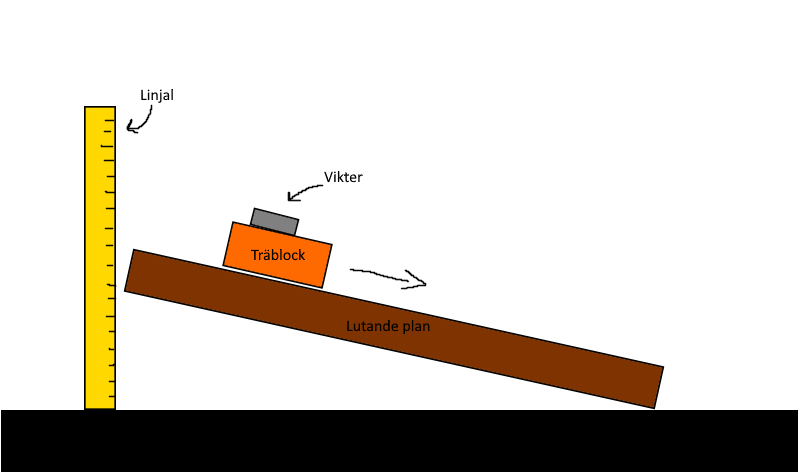
\includegraphics[width=0.8\textwidth]{images/lutandeplangrej}
            \caption{Experiment 1}
            \label{fig:lutandeplan}
        \end{figure}

        \begin{figure}[!h]
            \includegraphics[width=0.8\textwidth]{images/fjäder}
            \caption{Experiment 2}
            \label{fig:fjäder}
        \end{figure}

    \newpage
	\section{Analys och beräkning: Experiment 1}
        Datat från experiment 1 visas i tabell \ref{table:result}
        
        \begin{table}
            \begin{center}
            \begin{tabular}{ |c|c| } 
                \hline
                Massa (kg) & Höjd på planka (cm)  \\
                \hline
                0,1946 & 22,6 \\
                0,2446 & 21,2 \\
                0,2946 & 20,4 \\
                0,3446 & 19,4 \\
                0,3946 & 19,6 \\
                \hline
            \end{tabular}
                \caption{Mätvärden från experiment 1}
                \label{table:result}
            \end{center}
        \end{table}

\begin{table}
    \begin{center}
        \begin{tabular}{ |c|c| }
            \hline
            Friktionskraft (N) & Normalkraft (N)  \\
            \hline
            -0,53985 & -1,83313 \\
            -0,63652 & -2,3161 \\
            -0,73771 & -2,79733 \\
            -0,82061 & -3,28297 \\
            -0,94937 & -3,75687 \\
            \hline
        \end{tabular}
        \caption{Resultaten från experiment 1}
        \label{table:result1.1}
    \end{center}
\end{table}

Datat importeras i Excel och friktionskraften beräknas med hjälp av formeln:
    \begin{equation}
        F = {m}\cdot{g}\cdot{\sin(a)}
    \end{equation}
    Och Normalkraften beräknas med formeln:
    \begin{equation}
        F_N = {m}\cdot{g}\cdot{\cos(a)}
    \end{equation}
    Tabell \ref{table:result1.1} visar resultaten sammanställda i en tabell.
    Bild \ref{fig:graf1} visar resultaten sammanställda i en graf.

        \begin{figure}[!h]
            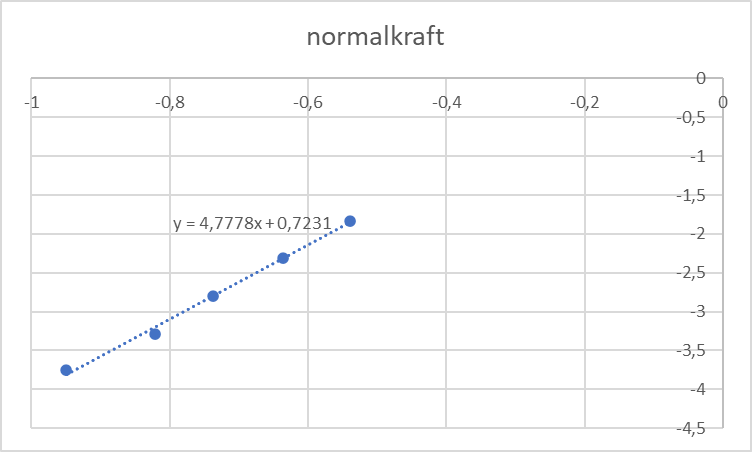
\includegraphics[width=0.8\textwidth]{images/lutandeplangraf}
            \caption{Normalkraften i newton (y) beror på friktionskraften i newton (x). I detta fall kan vi se att lutningskoefficienten är = 4,7778, vilket innebär att för varje newton i friktionskraft så ökar normalkraften med 4,7778 newton.}
            \label{fig:graf1}
        \end{figure}

        \section{Analys och beräkning: Experiment 2}
        Datat från experiment 2 visas i tabell \ref{table:result2}

\begin{table}
    \begin{center}
        \begin{tabular}{ |c|c| }
            \hline
            Massa (kg) & Längd på fjäder (cm)  \\
            \hline
            0 & 5,5 \\
            0,05 & 9,7 \\
            0,1 & 17 \\
            0,15 & 24 \\
            0,2 & 31 \\
            \hline
        \end{tabular}
        \caption{Mätvärden från experiment 2}
        \label{table:result2}
    \end{center}
\end{table}

\begin{table}
    \begin{center}
        \begin{tabular}{ |c|c| }
            \hline
            Fjäderkraft (N) & Elongation (m)  \\
            \hline
            0 & 0 \\
            0,491 & 0,042 \\
            0,982 & 0,115 \\
            1,473 & 0,185 \\
            1,964 & 0,255 \\
            \hline
        \end{tabular}
        \caption{Resultaten från experiment 2}
        \label{table:result2.1}
    \end{center}
\end{table}


        Datat importeras i Excel och fjäderkraften beräknas med hjälp av formeln:
        \begin{equation}
            F = {m}\cdot{g}
        \end{equation}
        Tabell \ref{table:result2.1} visar resultaten sammanställda i en tabell.
        Bild \ref{fig:graf2} visar resultaten sammanställda i en graf.

        \begin{figure}[!h]
            \includegraphics[width=0.8\textwidth]{images/fjädergraf}
            \caption{Elongationen av fjädern i cm (y) beror på fjäderkraften i newton (x).}
            \label{fig:graf2}
        \end{figure}
    
    \section{Slutsats och resultat} 
        Resultatet av beräkningarna illustreras i bilderna \ref{fig:graf1} och \ref{fig:graf2}.
    \section{Diskussion} 
    Resultatet är kanske inte helt perfekt på grund av vårat utförande. I början var vi lite mer slarviga med våra mätningar så trovärdigheten av mätvärdena kan ifrågasättas. Annars tycker jag att mätningarna för det mesta verkar rimliga.


    
    \printbibliography

\end{document}

